
\chapter{基于随机森林的统计翻译在线学习方法}
\label{Chapter_online}

近年来,统计机器翻译的研究发展迅速,翻译性能不断提高,在某些特定领域和环境下已经开始投入实际应用。但是,基于翻译记忆的计算机辅助翻译软件仍具有得天独厚的优势。随着机器翻译技术的不断发展,虽然通过引入机器翻译来辅助专业译员以提高人工翻译效率是行业的必然趋势,但在很多时候,专业译员往往不想花费太多时间阅读自动译文。

经过调研和分析,我们发现至少有两方面的原因造成了当前的现状。一方面,在特定领域中,如果待翻译文本与记忆库中的文本匹配程度很高时,译文质量明显优于机器翻译的译文。另一方面,随着翻译任务的进行,翻译记忆可以实时更新,而机器翻译一直重复相同错误。因此,如果能充分利用人工翻译句子中的翻译知识,并实时更新人机交互式翻译模型,就能显著提升自动译文的质量,进而增强机器翻译的可用性。
人们期待机器翻译系统能通过人机交互过程中的在线学习来改善后续自动译文。我们知道某些短语会被机器翻译错误地翻译,如果不及时纠正,在将来会重复出现相同的错误。因而如何避免重复相同错误是机器翻译的一个重要问题。在面向人机交互式的机器翻译系统中,随着翻译项目的进行,机器翻译系统的在线学习是一项核心任务。在线学习算法从用户反馈的人工翻译句子中发掘新的翻译知识,并实时更新模型,最终得到质量更好的自动译文。简而言之,人机交互式机器翻译系统的在线学习就是利用人工翻译句子实时改进后续自动译文以尽可能避免重复相同错误。

本章关注人机交互式机器翻译系统中最重要的统计翻译模型。在本章中,为了充分利用译员已完成的双语句对,我们提出了一种基于随机森林的统计翻译在线学习方法。该方法通过在人机交互过程中实时从输入源文和用户反馈构成的平行句对中抽取翻译知识,不断更新基于随机森林的统计翻译模型,从而改善译文的质量。由于低频词和未登录词直接影响词对齐和翻译知识抽取的性能,我们还提出了一种基于锚点的隐马尔可夫增量式词对齐方法。该词对齐方法有效利用互信息和词典等先验知识生成对齐锚点,然后联合执行基于锚点的双语短语划分和隐马尔可夫词对齐算法。

以图\ref{Fig_online_overview}中所示的英中翻译任务为例,在翻译第一句时,原文中的术语“publi-cation chair”被机器翻译系统错误地译成了“出版物的椅子”。而在翻译第二句时,人名“Hitoshi Isahara”的机器翻译结果也不是我们期望的正确结果。如果所使用的机器翻译系统没有学习回路,当翻译第三句时,“publication chair”和“Hitoshi Isahara”两个短语会继续被错误翻译,如第三句的机器翻译结果所示。

但在用户反馈的人工译文的帮助下,我们提出的基于随机森林的统计翻译在线学习方法在译员完成第一句的翻译之后,便进入学习回路:先通过基于锚点的隐马尔可夫增量式词对齐方法学习到译员已将第一句的上下文中的“chair”翻译成了“主席”,然后将新抽取到的翻译规则更新到基于随机森林的翻译模型中。同理,当第二句被翻译完成之后,我们提出的词对齐方法成功将未登录词“Hitoshi Isahara”对齐到正确的中文翻译“井佐原均”,同时将新抽取到的人名翻译更新到翻译模型中。因此当译员翻译第三句时,所使用的机器翻译系统已完成两个周期的在线学习过程。更新后的机器翻译系统再次遇到译员纠正过的源语言短语时,就可能输出正确的翻译结果,如图\ref{Fig_online_overview}中的第三句所示。根据图\ref{Fig_online_overview}中第三句的机器翻译自动译文,我们可以看到翻译质量得到了明显提高。

\begin{figure}[!tb]
	\centering
	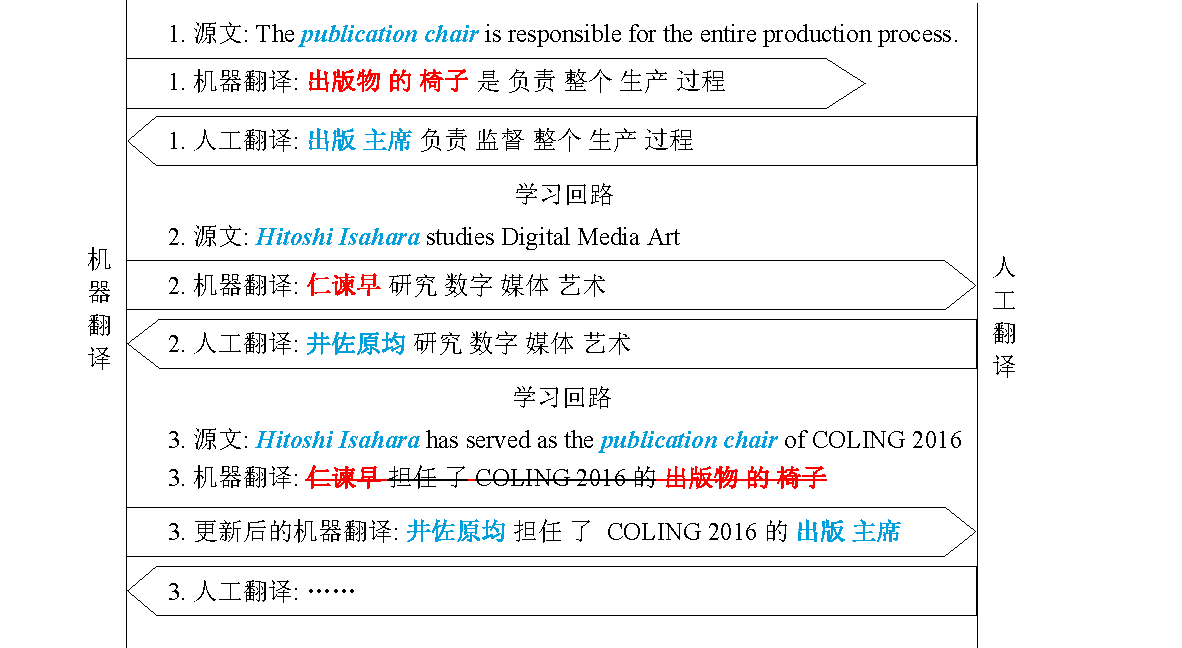
\includegraphics[width=0.95\textwidth]{Figure/Figure_5_1.pdf}
	
	\leftline{\qquad \ 正确的关键短语翻译:}
	
	“publication chair” ||| “出版主席”、“Hitoshi Isahara”||| “井佐原均”
	\caption{统计翻译模型在线学习概览图}
	\label{Fig_online_overview}
\end{figure}

通过使用基于随机森林的统计翻译在线学习方法和基于锚点的隐马尔可夫增量式词对齐方法,我们期望统计机器翻译系统能够学习到用户反馈的翻译知识来改善自动译文的质量。

本章的组织结构如下:5.1节介绍基于随机森林的统计翻译模型,然后在5.2节中讨论统计翻译模型的在线学习方法;5.3节详细介绍基于锚点的隐马尔可夫增量式词对齐方法;5.4节介绍已有相关工作;5.5节给出实验和分析,最后的5.6节对本章进行总结。

\section{基于随机森林的统计翻译模型}

近些年,将随机森林(Random forests, RFs)[\cite{Breiman:2001}]用于自然语言处理[\cite{Xu:2004}]任务中吸引了越来越多研究者的兴趣。已有证据显示,随机森林的分类性能好于或者至少可比于当前其它最先进的方法[\cite{Breiman:2001,Bosch:2007}]。对于机器翻译而言,随机森林的以下优势使得它非常适合建立翻译模型:(1)决策树的训练和测试都很快;(2)很容易做到大规模并行,因为森林中的每棵树的构建和测试过程都是独立于其它树的;(3)决策树天生适合多分类任务,这恰好对应于翻译模型中一个源语言短语有多个目标语言短语。除此之外,相对于Boosting或者其它集成学习方法而言,随机森林能更好地对抗噪声[\cite{Breiman:2001}]。

在本文中,我们首先建立基于随机森林的短语翻译模型。相对于文献\cite{Koehn:2003}]中的短语翻译模型而言,基于随机森林的短语翻译模型在解码过程中,能更好地结合上下文信息来选择短语翻译规则。基于随机森林的短语翻译模型是一种基于判别式方法的翻译模型,类似于文献[\cite{He:2008,LiuQun:2008}]介绍的方法。受文献[\cite{Saffari:2009}]的启发,我们将提出的基于随机森林的短语翻译模型作为接受用户反馈进行在线学习的起点。

\begin{figure}[!tb]
	\centering
	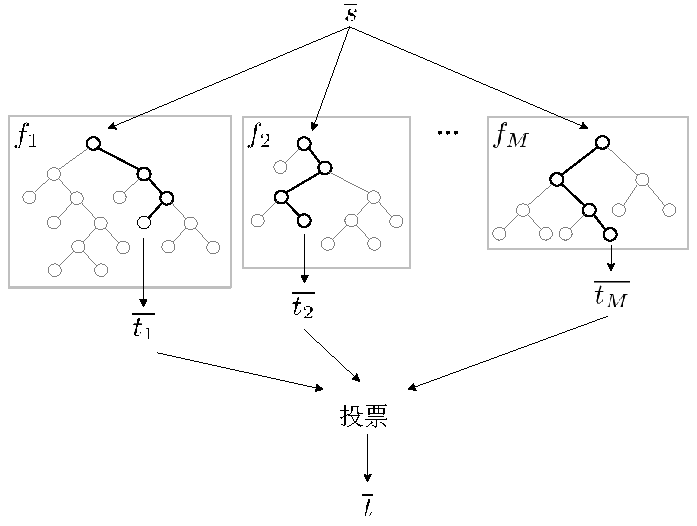
\includegraphics[width=0.9\textwidth]{Figure/Figure_5_2.pdf}
	\caption{统计翻译基于随机森林的短语翻译模型}
	\label{Fig_random_forests}
\end{figure}

如图\ref{Fig_random_forests}所示,在短语翻译模型中,源短语$\overline{s} $对应的随机森林为$\mathcal{F} = \{ f_1,f_2,\ldots,f_M \}$,其中$M$为随机森林中决策树的数量;第$m$棵决策树表示为$f(\overline{s},\theta_m): \mathcal{S} \to \mathcal{T}$,其中,$\theta_m$表示该决策树的参数向量。根据随机森林$\mathcal{F}$,若给定源语言短语$\overline{s}$,则目标短语$\overline{t}$的翻译概率为:

\begin{equation}\label{rf_trans_prob}
p(\overline{t}|\overline{s}) = \frac{1}{M} \sum_{m=1}^{M}p_m (\overline{t}|\overline{s})
\end{equation}

随机森林的构建是在抽取短语翻译规则表之后进行的,因此随机森林的训练集就是抽取的带上下文信息的短语翻译规则表。由公式\ref{rf_trans_prob}可知,翻译模型的随机森林中的每棵决策树是相互独立的:独立构建,独立测试。在随机森林的训练阶段,使用Bagging方法,每棵决策树接收到不同的、从原始训练集放回抽样的自举训练集,然后利用自举训练集分别构建决策树。Bagging方法也叫自举汇聚法(bootstrap aggregating),是一种在原始数据集上通过有放回抽样重新选出新数据集来训练分类器的集成技术。也就是说这些新数据集是允许重复的。

我们将随机森林训练集中未被抽样作为树$f_m$的自举训练集成员的样本称为集外样本(out-of-bag samples,OOB samples)。集外样本可以用来计算树$f_m$的集外样本错误率(out-of-bag-error,OOBE)。决策树中的每个节点的决策因子可形式化为$g(x) > \theta$,通常包含两部分:(1)决策函数$g(x)$,预先定义一系列函数模板,然后随机生成决策函数;(2)阈值$\theta$,按特征的值将样本分给左孩子节点或者右孩子节点的依据。

为了给决策树中的一个节点选择最佳的决策因子,首先随机生成一批决策因子候选,然后根据落在该节点的训练集$\mathcal{R}_j$的熵确定最佳的候选:
\begin{equation}
L(\mathcal{R}_j)=-\sum_{\overline{t}=1}^{\overline{T}} p_{\overline{t}}^j \log(p_{\overline{t}}^j)
\end{equation}
其中,$p_{\overline{t}}^{j}$表示目标短语$\overline{t}$在节点$j$处的比例,$\overline{T}$为训练集中目标短语的数量。

具体而言,在节点$j$被创建时,我们将首先按函数模版随机生成数目为$N$的决策因子集合$\mathcal{S} = \{(g_1(x), \theta_1), \ldots, (g_N(x), \theta_N)\}$。对于节点$j$,随机选择一个决策因子$s=(g'(x),\theta')$后,训练集中的样本将被分成两个集合$\mathcal{R}_{jls}$和$\mathcal{R}_{jrs}$。使$g'(x)\ge \theta'$成立的样本将被放入集合$\mathcal{R}_{jrs}$中,否则将被放入集合$\mathcal{R}_{jls}$中。则该划分$d$的信息增益$\triangle L(\mathcal{R}_j,\overline{s})$可由下式计算得到:
\begin{equation}
\Delta L(\mathcal{R}_j,d) = L(\mathcal{R}_j) - \frac{|\mathcal{R}_{jls}|}{|\mathcal{R}_j|}L(\mathcal{R}_{jls}) - \frac{|\mathcal{R}_{jrs}|}{|\mathcal{R}_j|}L(\mathcal{R}_{jrs})
\end{equation}
其中,$\mathcal{R}_{jls}$和$\mathcal{R}_{jrs}$分别表示被决策因子$s$分到左孩子和右孩子节点的训练样本集合,$|\cdot|$表示集合中元素的个数。一个决策因子确定的划分的信息增益越大,表明选定的划分函数和划分阈值越优,意味着得到更好的样本划分,同时也表明该节点的噪声越小。

借鉴文献[\cite{He:2008,LiuQun:2008}]利用判别式模型对翻译规模进行分类的经验,我们为每条短语翻译规则设计了如下十一类特征:

\begin{enumerate}[(1)]
	\item 短语翻译对中,源语言短语之前的六个词,表示为$WS_{s-6},\ldots,WS_{s-1}$;
	
	\item 短语翻译对中,源语言短语之后的六个词,表示为$WS_{s+1},\ldots,WS_{s+6}$;
	
	\item 短语翻译对中,源语言短语第一个词,表示为$WSL_s$;
	
	\item 短语翻译对中,源语言短语最后一个词,表示为$WSR_s$;
	
	\item 短语翻译对中,目标语言短语第一个词, 表示为$WSL_t$;
	
	\item 短语翻译对中,目标语言短语最后一个词, 表示为$WTL_{t}$;
	
	\item 短语翻译对中,目标语言短语之前的一个词, 表示为$WTL_{t-1}$;
	
	\item 短语翻译对中,目标语言短语之后的一个词, 表示为$WTL_{t+1}$;
	
	\item 源短语与目标短语的正向和反向词汇化翻译概率, 表示为$P_w(t|s)$和$P_w(s|t)$;
	
	\item 该短语翻译对是否被译后编辑采用,表示为$PS=1$或$PS=0$;
	
	\item 短语翻译对中,源语言短语和目标语言短语的长度,分别表示为$Len_s $和$Len_t$。
\end{enumerate}

以从英汉双语句对$<s=$“The publication chair is responsible for the entire production process .”$,t=$ “NULL\{1,4,7\} 出版\{2\} 主席\{3\} 负责\{5,6\} 监督\{\} 整个\{8\} 生产\{9\} 过程\{10\} 。\{11\}”$>$抽取出的短语翻译对$<\overline{s}=$“chair”,$\overline{t}=$“主席”$>$为例,符号“\{\}”之内的数字为目标语言词到源语言词的双语词对齐,这十一类特征分别为:

\begin{enumerate}[(1)]
	\item 源语言短语之前的六个词分别为:$WS_{t-6} =$ SENT\_BEFORE\_BEGIN、 $WS_{t-5} =$ SENT\_BEFORE\_BEGIN、 $WS_{t-4} =$ SENT\_BEFORE\_BEGIN、 $WS_{t-3} =$ SENT \_BEGIN、 $WS_{t-2} =$ the、 $WS_{t-1} =$ publication。 其中,SENT\_BEGIN表示句子开始符, SENT\_BEFORE\_BEGIN表示句子开始之前的空白占位符。
	
	\item 短语翻译对中,源语言短语之后的六个词分别为:$WS_{t+1}=$ is、$WS_{t+2}=$ responsible、$WS_{t+3}=$ for、$WS_{t+4}=$the、$WS_{t+5}=$ entire、$WS_{t+6}=$ production。
	
	\item 源语言短语第一个词:$WSL_s=$ chair。
	
	\item 源语言短语最后一个词:$WSR_s=$ chair。
	
	\item 目标语言短语第一个词:$WTL_s=$ 主席。
	
	\item 目标语言短语最后一个词:$WTR_s=$ 主席。
	
	\item 目标语言短语之前的一个词:$WTL_{t-1}=$ 出版。
	
	\item 目标语言短语之后的一个词:$WTR_{t+1}=$ 负责。
	
	\item 源短语与目标短语的正向和反向词汇化翻译概率, 表示为$P_w(t|s) = 0.45892387$ 和 $P_w(s|t) = 0.6623509$;
	
	\item 该短语翻译对是否被译后编辑采用,表示为$PS=1$;
	
	\item 源语言短语和目标语言短语的长度:$Len_s=1$和$Len_t=1$。
\end{enumerate}

为了利用基于随机森林的翻译模型进行翻译,我们将构建完成的翻译模型融合到统计机器翻译解码器的对数线性模型之中。在本文中,对数线性模型包含的特征为:利用基于随机森林的翻译模型计算的正向翻译概率$p(t|s)$和反向翻译概率$p(s|t)$、正向词汇化翻译概率$lex(t|s)$和反向词汇化翻译概率$lex(s|t)$、语言模型、基于最大熵的调序模型、目标端单词数惩罚因子和短语数惩罚因子。

\section{基于在线随机森林的统计翻译在线学习方法}

上一节介绍的基于随机森林的机器翻译模型主要用于离线学习(off-line learning)或者批量学习(batch learning)。批量学习要求训练数据在学习之前一次性得到以满足批量性,即在构建每一棵决策树时,用于本次学习的批量训练集是可见的[\cite{LiLijia:2010}]另外也有针对决策树的增量学习(incremental learning)方法,即每次学习一个或多个样本,这些训练样本可以全部保留、部分保留或不保留。但目前已有的方法并不能满足机器翻译在线学习场景,如每个节点都必须看到或者存储所有训练子集[\cite{Utgoff:1997}],或者当父节点更新时的代价过大从而导致分类性能的急速下降。

本文的在线学习(online learning)主要指动态学习的过程,根据用户反馈不断地修正和优化模型,包括增量学习和递减学习(decremental learning)。递减学习指在训练过程中会抛弃“价值最低”的已学到的部分参数和已保留的训练样本。

为了使基于随机森林的机器翻译模型实现在线学习,我们面临两个主要问题:(1)如何将Baging方法应用于在线机器翻译模型;(2)如何在线动态构建和修正决策树。随机森林是由一系列通过Bagging方法训练得到的随机决策树组成的。所以,随机森林的在线学习版本需将在线Bagging方法[\cite{Oza:2005}]与在线随机决策树融合在一起。其中,在线随机决策树在构建过程中随机选择特征。

\subsection{在线Bagging}

人机交互式翻译过程符合在线学习协议(online learning protocol)[\cite{Cesa-Bianchi:2006}],译员完成的人工翻译译文一句接一句像流水一样反馈到机器翻译系统中,如图\ref{Fig_online_overview}所示。对每个源语言句子而言,机器翻译系统会输出一句自动译文。随后,译员通过修改自动译文或者直接翻译来完成最终译文。这样,在译员开始翻译下一句源语言句子之前,机器翻译系统有一个执行学习回路的时间间隔。在学习回路中,先执行词对齐,然后抽取出一系列短语翻译规则并更新翻译模型。

在本文中,我们将实时抽取出的短语翻译规则看作随机过程,并且用泊松分布模拟翻译规则的到达。当一条翻译规则到达时,我们将用这条规则依次更新源语言短语对应的随机森林中的所有决策树。因此,决策树 会被这条规则更新 次。其中, 由符合泊松分布的随机数发生器生成[\cite{Oza:2005}]。

\subsection{在线随机决策树}

本文中,我们采用了极度随机森林(extremely randomized forests)算法[\cite{Geurts:2006}]来构建基于在线随机森林的统计翻译模型。极度随机森林是由一系列极度随机决策树组成,它具有调整参数少、计算速度快、抗噪性能好以及可克服维数灾难等优点。所谓极度随机森林,指决策因子$g(x) < \theta$中的决策函数$g(x)$和阈值$\theta$均通过随机选择确定。因此,在本文中,基于在线随机森林的统计翻译模型中的在线随机决策树的构建过程,就是极度随机决策树的构建过程。

离线学习模式中,构建决策树时,每个节点都能看到所有落在该节点的训练子集。因此,该节点对训练子集的全部样本计算信息增益等统计量。经过充分评估后,可以选择全局最合适的决策函数和阈值。但是在在线学习模式中,训练样本随着时间依次到来,相关统计量是动态变化的。

就单个节点而言,是否需要划分主要依赖于两点:是否已经积累了足够的样本以确保得到鲁棒的统计量;当前的划分性能是否已达到足够好的程度。为此,我们将引入两个超参数:划分之前,落入该节点的最小样本数阈值$\alpha$;划分之后的最小信息增益阈值$\beta$。

在本文中,当且仅当如下条件成立时,在线随机决策树的节点才对落入的样本进行划分:$|\mathcal{R}_j| > \alpha$并且$\exists d \in \mathcal{S}: \Delta L(\mathcal{R}_j,d) > \beta$。即如果样本数量$|\mathcal{R}_j|$超过最小样本数阈值$\alpha$,并且信息增益超过最小信息增益阈值$\beta$,则通过决策因子$(g(x),\theta)$确定最佳划分,否则将短语翻译对的源语言短语、目标语言短语和短语翻译对对应的上下文特征信息存入所述决策树叶节点$j$,即添加至训练集$\mathcal{R}_j$。

\subsection{动态加权}

\begin{figure}[!tb]
	\centering
	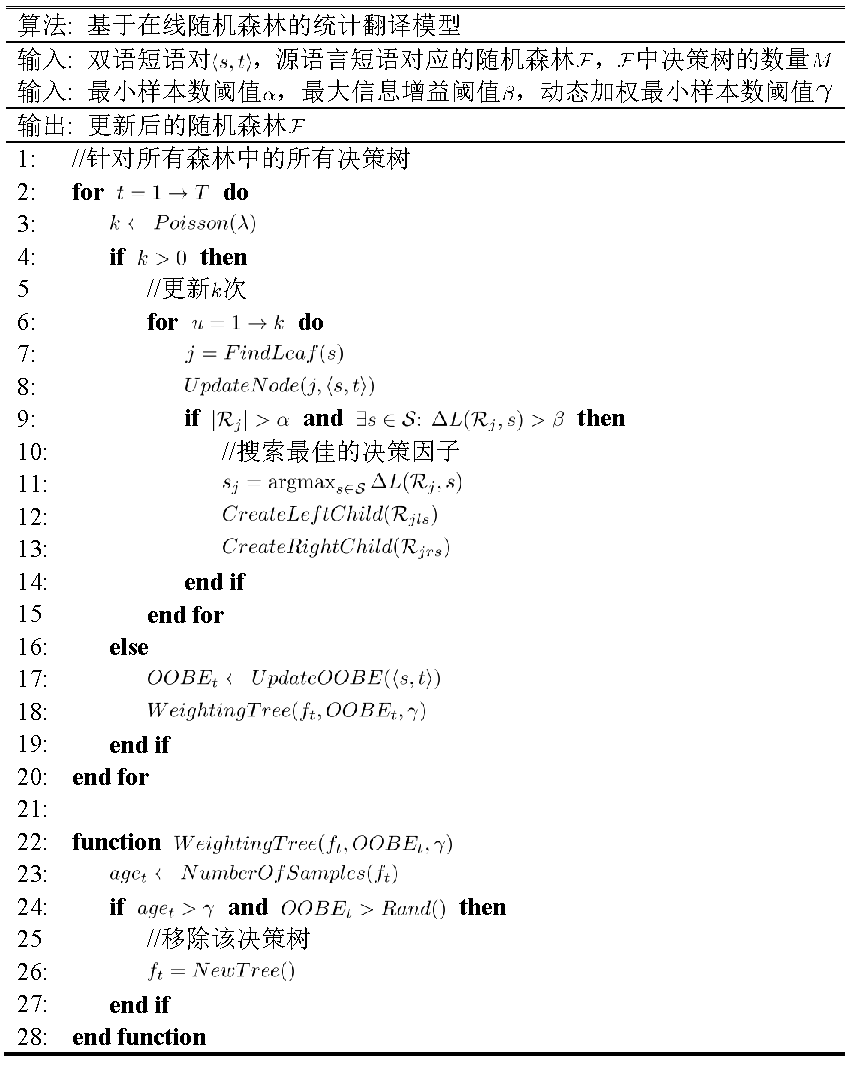
\includegraphics[width=0.95\textwidth]{Figure/Figure_5_3.pdf}
	\caption{基于在线随机森林的统计翻译模型在线学习算法}
	\label{Fig_online_algorithm}
\end{figure}

在人机交互式机器翻译场景中,翻译任务的领域或者上下文会随着时间发生变化,这就要求机器翻译系统对未来的翻译任务有很强的适应能力。而传统机器翻译系统的“一次离线训练,长时间使用”并不能满足随时可能变化的翻译任务,如果进行增量式学习,大量的老旧训练样本会淹没新样本。为了提升在线随机森林的统计翻译模型的适应能力,我们为在线随机森林引入动态加权的方法:在适当的时候,在线随机森林将分类性能较低的随机决策树删除,并收集新的训练样本以重新构建处理相同特征的决策树。

为了达到动态加权的目的,在一条翻译规则到达之后、更新决策树 之前,如果Bagging随机数发生器的结果为0,则我们首先将这条翻译规则加入到该决策树的集外样本集中,而不用该样本更新该决策树。然后利用该决策树已累积的集外样本计算决策树$f_t(x)$的集外样本分类错误率$OOBE$。如果集外样本错误率$OOB$大于临时生成的随机数(0.1到1之间的小数)且该决策树接收到的所有样本数量$age$超过了动态加权最小样本数阈值$\gamma$,则从对应的随机森林中移除该决策树。

综上所述,完整的基于在线随机森林的统计翻译模型在线学习算法如图\ref{Fig_online_algorithm}所示。随着用户反馈的人工翻译句子的增多,翻译模型中质量比较差的决策树将被移除,同时生成分类能力更强的决策树。因此,翻译模型的准确率将逐步增强。

在本文中,最小样本数阈值$\alpha$的默认值为30,最大信息增益阈值$\beta$的默认值为0.1,动态加权最小样本数$\gamma$的默认值为50。

\subsection{案例研究}

基于在线随机森林的统计翻译模型在线学习的步骤为:

(1)获得双语词对齐信息,抽取短语翻译对及其上下文特征信息。

(2)逐对更新源语言短语相关的翻译模型随机森林。

(3)根据短语翻译对及其上下文特征信息,得到随机森林中的决策树的测试错误率,如果超过测试错误率阈值则移除对应的决策树。

现举例说明$\{WS_{t-2},WS_{t-1}\}$决策树的构建过程:

(1)起始为空树,只有根结点。

\begin{figure*}[!h]
	\centering
	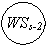
\includegraphics{Figure/Figure_5_0_1.pdf}
\end{figure*}

(2)反馈下列句对之后的决策树为:

A. The man sat down in the chair by the fire and put his gun away.

那人在炉火边的椅子里坐下,把枪收了起来。

B. A man would pull out the woman's chair in a restaurant.

在餐厅里,男人会细心地为女人拉开椅子。

C. He, on his chair, scarcely looks at her and smokes ceaselessly.

他坐在椅子上,不怎么看她,只是不停地抽烟。

\begin{figure*}[!h]
	\centering
	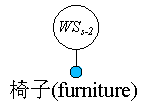
\includegraphics{Figure/Figure_5_0_2.pdf}
\end{figure*}

(3)反馈下列句对之后的决策树为:

D. Prof. Jones holds the chair of phonetics.
琼斯教授担任语音学讲座。

\begin{figure*}[!h]
	\centering
	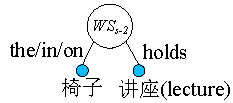
\includegraphics{Figure/Figure_5_0_3.pdf}
\end{figure*}

(4)继续反馈下列句对之后的决策树:

E. The publication chair is responsible for the entire production process.
出版主席负责监督整个生产过程。

\begin{figure*}[!h]
	\centering
	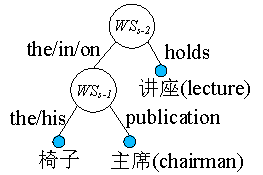
\includegraphics{Figure/Figure_5_0_4.pdf}
\end{figure*}

由上述过程可知,短语翻译对的抽取依赖词对齐结果。在在线学习场景中,为了避免因集外词对词对齐的影响,我们将提出基于锚点的增量式词对齐的方法。

\section{基于锚点的隐马尔可夫增量式词对齐方法}

在统计机器翻译任务中,找到词对应关系之后,才能抽取翻译规则。因此,词对齐任务扮演着非常重要的作用。令源语言句子为$S=s_1^J=s_1s_2\ldots s_J$,目标语言句子为$T=t_1^I=t_1t_2\ldots t_I$,其中,$J$和$I$分别为源语言句子和目标语言句子的单词数。词对齐任务可看作是搜索最佳双语词对应序列$A=a_1a_2\ldots a_J$的任务,其中$a(j)=i$表示目标语言句子中的第$i$个词$t_i$对应于源语言句子的第$j$个词$s_j$。在统计机器翻译任务中,为了得到较好的词对齐结果,现在的标准做法是结合IBM模型1-5[\cite{Brown:1993}]、基于隐马尔可夫的词对齐方法[\cite{Vogel:1996}]和IBM模型6[\cite{Och:2003b}]。

但是,在人机交互式翻译过程中,译员不断地反馈新的双语平行句对,在线机器翻译模型必然要求词对齐模型也能尽快学习到新的翻译知识,从而不断降低词对齐错误率。在人机交互式翻译场景中,词对齐任务主要面临两方面的挑战。最大的挑战是未登录词和已知词的低频译文。数据稀疏问题和长尾效应使得我们很难实时纠正对齐错误,从而进一步影响当前句对的翻译知识抽取。另一个挑战是长句会极大地降低词对齐性能,包括对齐时间和对齐准确率。在离线训练机器翻译时,我们可以简单地过滤掉词数过多的双语句对,但在人机交互式场景中,我们不能这样做。因为在实际翻译任务中,译员反馈的人工翻译句子非常宝贵,简单过滤后可能造成进一步的数据稀疏。

因此,在本文中,我们关注增长式实时双语词对齐的方法,即要求很快给出词对齐结果以便抽取新的翻译规则,同时还要能动态增加训练语料以进一步降低词对齐错误率。

通常而言,当前的增长式双语词对齐性能并没有达到能直接用于统计机器翻译实时学习新翻译知识的水平(参见http://www.statmt.org/moses/?n =Advanced.Incremental)。其主要原因为如下四点:(1)对新词处理能力较弱;(2)长句的词对齐错误率较高;(3)大规模语料的训练周期仍然较长;(4)未充分利用置信度较高的先验知识。如果直接将先验知识作为词对齐的约束,并不能带来性能的提升,还需要改进现有增长式双语词对齐算法。因此,研究如何利用先验知识,大幅减少增长式双语词对齐的训练时间,同时明显降低新词和长句的双语词对齐的错误率,并提高最终的机器翻译译文质量是迫切需要解决的一个难题。

经过分析,在人机交互式翻译过程中,我们有如下发现:

(1)由于新增加的平行句对中可能出现新词,因此利用互信息、领域词典等先验知识作为双语词对齐的起点,有利于降低新词的词对齐错误率。从而提高翻译规则抽取的准确率,最终提高机器翻译译文质量;

(2)通过先进行双语短语切分,再搜索短语内部词对齐,能有效降低长句的双语词对齐错误率;

(3)在一次批处理更新周期内,仅更新出现次数小于词更新阈值的源语言词和目标语言词的翻译概率,有利于大幅降低训练周期,满足增长式实时双语词对齐的要求。

基于以上观察,我们提出一种基于锚点的隐马尔可夫增量式词对齐方法,降低增长式双语词对齐的训练时间,同时提高新词和长句的双语词对齐性能,并提高最终的机器翻译译文质量。该词对齐方法的基本思想是利用先验知识生成词对齐锚点,有效降低新词和长句的词对齐错误率,同时降低增量式词对齐的时间复杂度,有效提升了增长式实时词对齐的可用性。

在下文中,我们结合图5.4所示的例子详细介绍提出的基于锚点的隐马尔可夫增量式词对齐方法,主要包括三个步骤:(1)搜索锚点;(2)根据锚点进行双语短语划分;(3)在双语短语划分的约束下搜索最佳词对齐结果。

\subsection{搜索锚点}

\textbf{(1)计算互信息}

在本文中,类似于文献[\cite{Zhang:2003}],我们利用互信息(mutual information,MI)来生成词对齐锚点。互信息的计划公式如下:
\begin{equation}
MI[s,t] = \log_2 \frac{P(s,t)}{P(s)P(t)}
\end{equation}
其中,$P(s,t)$指源语言词与目标语言词的共现频率:
\begin{equation}
P(s,t)=\frac{2\times count(s,t)}{count(s)+count(t)}
\end{equation}
$count(.)$表示出现次数,$P(s)$和$P(t)$分别为源语言词和目标语言词的出现频率。

图5.4(A)为词之间的互信息计算结果。互信息可以衡量两个变量之间相互依赖的强度。因此,一些互为翻译之间的词的互信息值相对较大,单元格的互信息值越大,对应词之间互为翻译的可能性也越大。如果源语言词和目标语言词都是首次出现,则相关互信息值则会明显超过周围单元格的值。

\textbf{(2)应用先验信息}

将最大互信息值对应的单元格或者其它先验知识标为锚点 。图5.4(A)中,最大的互信息值MI(“Netherlands”,“荷兰”)=8,则可以将“Netherlands”与“荷兰”作为对齐锚点。在本章中,词对齐先验知识包括:(1)领域词典;(2)领域术语库;(3)专家总结的双语词对齐规则。例如,可以根据词典查询到第一次出现的英语单词“disproportionately”的中文词为“特别 大”,则可以将“disproportionately”和“特别”或者“大”作为词对齐锚点,将MI(“disproportionately”,“特别”)或者MI(“disproportionately”,“大”)设置为8。

\textbf{(3)标记锚点}

标记上一步找到的锚点所对应的源语言句子词的下标为横坐标,将横坐标所在行的所有互信息替换为最小互信息值;同时标记这个锚点对应的目标语言句子词的下标为纵坐标,将纵坐标对应列的所有互信息替换为最小互信息值。

令原始锚点集合$H=H_1^M=\{h_m\}$,其中$h_m=(j,i)$表示源语言第$j$个词与目标语言第$i$个词构成的第$m$个对齐锚点,共$M$个锚点。

\begin{figure}[!hbt]
	\centering
	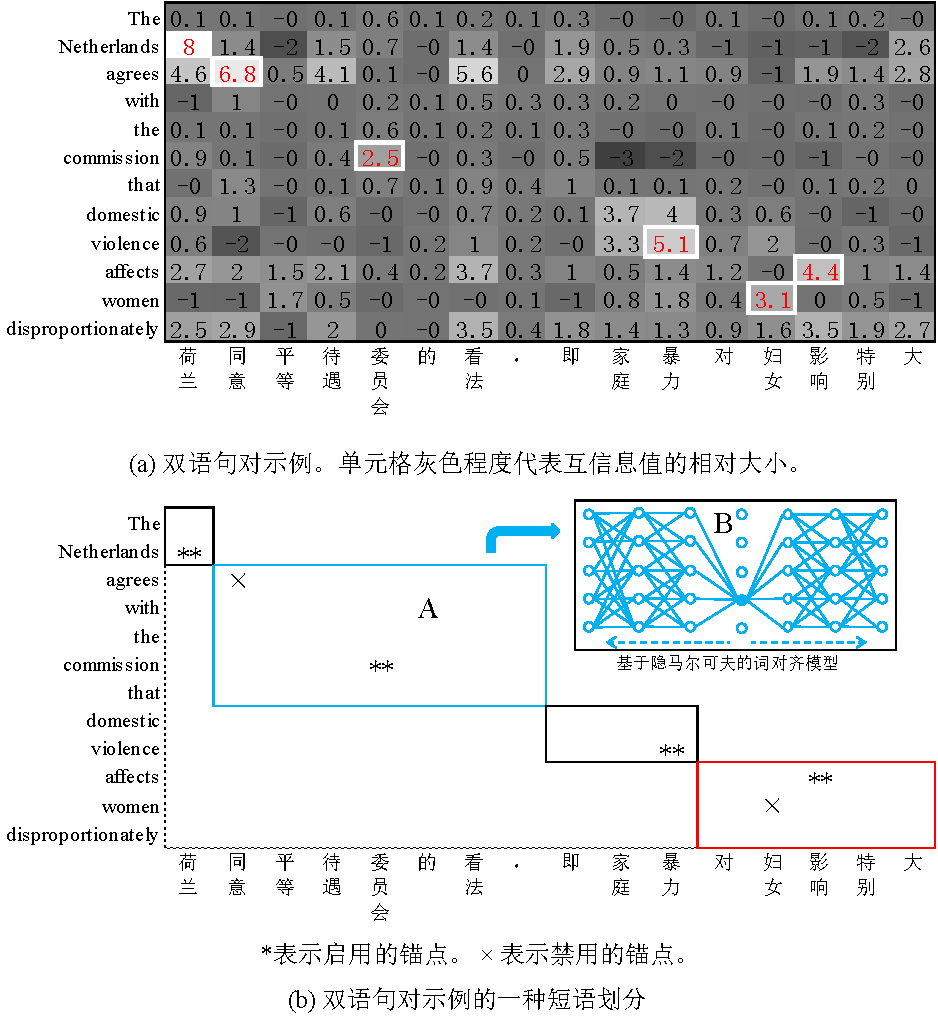
\includegraphics[width=0.96\textwidth]{Figure/Figure_5_4.pdf}
	\caption{基于锚点的隐马尔可夫增量式词对齐模型}
	\label{Fig_anchor_hmm}
\end{figure}

在图5.4(a)中,“Netherlands”与“荷兰”被确定为锚点后,源语言句子词
``Netherlands'' 的下标为2,目标语言句子词“荷兰”的下标为1,因此第一个锚点为$h_1=(2,1)$,然后将其加入到原始锚点集合$H$中。

在图5.4(a)的示例中,最小的互信息值MI(“commission”,“家庭”)=-3,因此将$h_1=(2,1)$加入原始锚点集合后,令所有MI(“Netherlands”,*)和MI(*,“荷兰”)的值为-3。

\textbf{(4)继续搜索锚点}

如果相邻锚点的横坐标或者纵坐标之间的最大距离超过距离阈值,则继续步骤(3),否则结束搜索锚点。
在本文中,最大距离阈值为7。图5.4(a)中最终可以确定6个锚点,分别为:(“netherlands”,“荷兰”)、(“agrees”,“同意”)、\linebreak
(“violence”,“暴力”)、(“affects”,“影响”)、(“women”,“妇女”)和(“com-mission”,“委员会”)。即锚点集合:
$$H=H_1^6=\{(2,1),(3,2),(9,11),(10,14),(11,13),(6,5)\}$$
经过采样分析,一般而言,锚点位置的词对齐准确率超过90\%。

\subsection{双语短语划分}

根据锚点集合$H$,我们对源语言句子和目标语言句子进行双语短语划分。令双语句子短语切分结果为$D=d_1d_2 \ldots d_N$,$d_n=(s.start, s.end, t.start, t.end, pa)$指第$n$个双语短语,$s.start, s.end, t.start, t.end$分别指源短语的起始下标、源短语的终止下标、目标短语的起始下标和目标短语的终止下标,$pa$为短语内双语词对齐。其中,双语短语词对齐$pa=a_1a_2\ldots a_{len(pa)}$,$a_j=\{i|a(j)=i\}$,其中$a(j)=i$指源语言短语第 个词与目标语言句子的第$i$个词对应, 可能有多个不同的值。在本文中,为简洁起见,令$d_n.pa = pa_n$。

以图5.4(b)为例,逐一遍历对齐锚点集合中的每个锚点,如$H_2=\{9,11\}$,则以该锚点为中心,在满足双语短语扩展约束的条件下,从源语言句子端和目标语言句子端分别向左右两边扩展,形成一个双语短语切分候选$d_3=(8,9,9,11,pa_3)$。如图5.4(b)中从左上角到右下角首尾连接的框,表示当前短语切分集合$D$包含四个双语短语切分候选:
$$D=\{(1, 2, 1, 1, pa_1), (3, 7, 2, 8, pa_2), (8, 9, 9, 11, pa_3), (10, 12, 12, 16, pa_4)\}$$

短语扩展时,为了避免因锚点错误造成的错误3传递,在探测过程中,每个锚点有启用(如图5.4(b)中的“**”)和禁用(如图5.4(b)中的“×”)两种状态。当相邻两个锚点之间的距离小于距离阈值时,该锚点可以被禁用。在一次探测过程中,被启用的锚点组成探测锚点集合$\widetilde{H}$。探测锚点集合$\widetilde{H}=\widetilde{H}_1^{N}=\{h_n\}$通过禁用部分锚点得到,是原始锚点集合的真子集,一次探测中,共$N$个锚点。图5.4(B)中的探测锚点集合为:$\widetilde{H}=\widetilde{H}_1^4 = \{(2,1), (6,5), (9,11), (11,13)\}$

双语短语扩展约束,指扩展时双语短语不能跨越启用的锚点,且双语短语的源语言端和目标语言端的长度均不能超过距离阈值,如本实施例中的阈值为7。双语短语扩展时,可以跨越已被禁用的锚点。如图5.4(b)中的A区域,短语扩展时就跨越了被禁用的锚点$(3,2)$。

\subsection{联合词对齐}

\textbf{(1)单句词对齐}

我们采用动态规划算法搜索最佳的双语短语切分,而在双语短语内部的词对齐可采用基本词对齐模型,如本文中的基于隐马尔可夫的词对齐模型[\cite{Vogel:1996}]。

就短语内的词对齐而言,根据隐马尔可夫词对齐模型假设,对于源语言短语位置$j$,对位$a_j$的概率对它前一个词的对位$a_{j-1}$具有一定的依赖性,即存在概率$P(a_j|a_{j-1},I)$。因此,双语短语词对齐模型$P(d_n.s,d_n.pa|d_n.t)$可以表示为:
\begin{equation}\label{phrase_word_align}
P(d_n.s_1^{J'},(pa_n)_1^{J'}|d_n.t_1^{I'})= \prod_{j=d_n.s.start}^{d_n.s.end} P((pa_n)_j|(pa_n)_{j-1},I') P(d_n.s_j|d_n.t_{(pa_n)_j})
\end{equation}
其中,$I'$和$J'$分别表示目标语言短语和源语言短语的长度,即词的数目。

原始的隐马尔可夫模型的初始状态为$a_0=0$,即源语言短语起始符对位目标语言短语起始符。在本章中,我们修改后的基于锚点的隐马尔可夫词对齐模型与文献[\cite{Vogel:1996}]的不同之处在于,本章中的隐马尔可夫模型的起始状态为词对齐锚点,如图5.4(a)中的锚点“commission”与“委员会”对应的$(6,5)$。因此,本章中的隐马尔可夫词对齐模型如图5.4(b)的B区域所示:竖排的空心圆点表示隐马尔可夫模型的内部状态序列,即中文短语对齐位置;实心点表示锚点,也是初始状态,即英文短语第4个词与中文短语第4个词,而锚点两边的词对齐直接依赖于短语切分中心的对齐锚点。因而,公式\ref{phrase_word_align}可进一步推导为:
\begin{equation}\label{phrase_word_align_further}
\begin{aligned}
P(d_n.s_1^{J'},(pa_n)_1^{J'}|d_n.t_1^{I'})= &  \prod_{j=h_n.s-1}^{1} P((pa_n)_j|(pa_n)_{j+1},I') P(d_n.s_j|d_n.t_{(pa_n)_j}) \\
& \times \prod_{j=h_n.s+1}^{J'} P((pa_n)_j|(pa_n)_{j-1},I') P(d_n.s_j|d_n.t_{(pa_n)_j})
\end{aligned}
\end{equation}

综上所述,令双语句子词对齐$A=pa_1pa_2\ldots pa_N$,最终双语句子词对齐$A^*$,最终锚点集合$H^*$和最终短语划分$D^*$,其中$N$指短语切分的数量。基于公式\ref{phrase_word_align_further},本章中提出的双语句子词对齐模型为:
\begin{equation}\label{anchor_hmm_word_align}
(A^*, H^*, D^*)= \mathop{\argmax}_{(s_1^J, t_1^I),\widetilde{H} \subseteq H}{\left[ \max \limits_{D} \prod_{n=1}^N P(d_n.s_1^{J'},(pa_n)_1^{J'}|d_n.t_1^{I'})\right]}
\end{equation}

公式\ref{anchor_hmm_word_align}将锚点探测、双语短语切分和短语内部词对齐融合在一起同时执行,在理论上避免了已有方法结合先验知识、长句对齐和新词处理存在错误相互传递的缺点。并且已有方法一般是独立进行先验知识的融合、长句切分成子句和新词处理,考虑到每个环节均可能引入错误而且会传递到下一阶段,最后可能造成词对齐性能的下降。

利用公式\ref{phrase_word_align_further}和\ref{anchor_hmm_word_align},图5.4(a)中对应的短语划分与对齐结果为:

$A=$\{荷兰\{netherlands\} 同意\{agrees\} 平等\{\} 委员会\{commission\} 的\{\} 看法\{with\} ,\{that\} 即\{\} 家庭\{domestic\} 暴力\{violence\} 对\{\} 妇女\{women\} 影响\{affects\} 特别\{disproportionately\} 大\{disproportionately\}\};

$\widetilde{H}=$\{(2, 1), (6, 5), (9, 11), (11, 13)\};

$D=$\{(the netherlands, 荷兰\{2\}), (agrees with the commission that, 同意\{1\} 平等\{\} 待遇\{\}  委员会\{4\} 的\{\} 看法\{2\} ,\{5\}), (domestic violence, 即\{\} 家庭\{1\} 暴力\{2\}), (affects women disproportionately, 对\{\} 妇女\{2\} 影响\{1\} 特别\{3\} 大\{3\})\}。

最终对齐结果为:

$A*=$\{荷兰\{netherlands\} 同意\{agrees\} 平等\{\} 委员会\{commission\} 的\{\} 看法\{with\} ,\{that\} 即\{that\} 家庭\{domestic\} 暴力\{violence\} 对\{\} 妇女\{women\} 影响\{affects\} 特别\{disproportionately\} 大\{disproportionately\}\};

$H*=$\{(2, 1), (6, 5), (9, 11), (11, 13)\};

$D*=$\{(the netherlands, 荷兰\{2\}), (agrees with the commission, 同意\{1\} 平等\{\} 待遇\{\}  委员会\{4\} 的\{\} 看法\{2\} ,\{5\}), (that domestic violence, ,\{1\} 即\{1\} 家庭\{2\} 暴力\{3\}), (affects women disproportionately, 对\{\} 妇女\{2\} 影响\{1\} 特别\{3\} 大\{3\})\}。

\textbf{(2)增量学习}

将源语言句子$s$、目标语言句子$t$和双语词对齐$A*$加入批处理训练集,如果批处理训练集大小超过阈值则更新词对齐模型,输出增量词对齐模型并替换现有词对齐模型。在本文中,批处理训练集最小阈值为500平行句对,即每累积500句对后就开始增量训练词对齐模型。

在增量学习过程中,我们使用类似于IncGiza++项目(https://code.google.com/ archive/p/inc-giza-pp/)采用的在线EM算法进行增量式词对齐。但为了加快迭代效率,在后续增量词对齐模型时,当累计平行句对超过500000句对时,我们不再更新隐马尔可夫模型的状态跳转概率。同时也不再更新源语言词和目标词共同出现次数超过30次的词翻译概率。即仅更新共现次数小于30次的源语言词和目标语言词的翻译概率。

鉴于本文所使用的基于锚点的隐马尔可夫模型不同于标准的隐马尔可夫词对齐模型,我们将在下一节讨论其推导过程。

\subsection{基于锚点的隐马尔可夫词对齐模型推导过程}

原始的隐马尔可夫模型的初始状态为$a_0=0$,本章中的隐马尔可夫模型的起始状态为预先确定的锚点。因更新隐马尔可夫模型的前向算法、后向算法和求解过程中的维特比算法不是本章的主要创新内容,且本章中的短语内词对齐并不限于使用隐马尔可夫词对齐模型,现简单说明更新隐马尔可夫模型的前向后向算法,具体计算细节可参见文献[\cite{zong:2013}]第6章第4节。

\textbf{(1)初始化}

在满足下列条件的情况下,随机初始化跳转概率$a_{ij}$和发射概率$b_j(k)$:
\begin{equation}
\sum_{j=1}^{N} a_{ij}=1, 1 \le i \le N
\end{equation}
\begin{equation}
\sum_{k=1}^{M} b_j(k)=1, 1 \le j \le N
\end{equation}

其中,$N$为隐马尔可夫模型中状态的数目(本文中取值为8),$M$为每个状态可能输出的不同符号的数目,即源语言词的数目。

\textbf{(2)迭代计算}

(2.1)由下列公式分别计算期望值$\xi_t(i,j)$和$\gamma_t(i)$。

给定隐马尔可夫模型的参数$\mu$和观察序列$O=O_1O_2\ldots O_T$,在时间$t$位置状态$s_i$的概率$\xi_t(i,j)=P(q_t=s_i,q_{t+1}=s_j | O, \mu)(1\le t \le T, 1 \le i,j \le N )$可以由下面的公式计算获得:

\begin{equation}
\begin{aligned}
\xi_t(i,j) & = \frac{P(q_t=s_i,q_{t+1}=s_j, O | \mu)}{P(O|\mu)} \\
& = \frac{\alpha_t(i)a_{ij}b_j(O_{t+1})\beta_{t+1}(j)}{P(O|\mu)} \\
& = \frac{\alpha_t(i)a_{ij}b_j(O_{t+1})\beta_{t+1}(j)}{\sum_{i=1}^{N}\sum_{j=1}^N \alpha_t(i)a_{ij}b_j()O_{t+1}\beta_{t+1}(j)}
\end{aligned}
\end{equation}

给定隐马尔可夫模型的参数$\mu$和观察序列$O=O_1O_2\ldots O_T$,在时间$t$位于状态$s_i$的概率$\gamma_t(i)$可以由下面的公式计算获得:
\begin{equation}
\gamma_t(i) = \sum_{j=1}^N \xi _t(i,j)
\end{equation}

其中,$\alpha_t(i)$是在时间$t$,隐马尔可夫模型输出了序列$O=O_1O_2\ldots O_t$,并且位于状态$s_i$的概率:
\begin{equation}
\beta_t(i)=P(O_{t+1}O_{t+2}\ldots O_T | q_t=s_i, \mu)
\end{equation}

(2.2)根据步骤(2.1)得到的期望值,根据下列公式重新估计参数$a_{ij}$和$b_j(k)$:
\begin{equation}
\overline{a}_{ij} = \frac{\sum_{t=1}^{T-1} \xi _t (i,j)}{\sum_{t=1}^{t-1} \gamma_t (i)}
\end{equation}
\begin{equation}
	\overline{b}_j (k) = \frac{\sum_{t-1}^T \gamma_t (j) \times \delta(O_t,v_k)}{\sum_{t=1}^T \gamma_{t} (j)} 
\end{equation}
其中,$v_k$表示输出第$k$个符号即源语言单词,$\delta(x,y)$为克罗奈克函数,当$x=y$时,$\delta(x,y)=1$,否则$\delta(x,y)=0$ 。

\textbf{(3)循环计算}

令$i=i+1$。重复执行(2),直到$a_{ij}$和$b_j(k)$收敛。

\section{实验}

\subsection{实验数据}

本文将在英中新闻翻译任务中来测试基于随机森林的统计翻译模型在线学习方法的性能。

\begin{figure}[t]
	\centering
	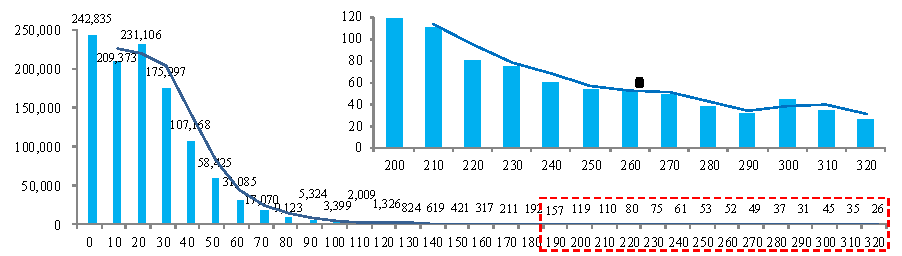
\includegraphics[width=0.98\textwidth]{Figure/Figure_5_5.pdf}
	\caption{句子长度直方图。横坐标表示句子长度,纵坐标表示句子数。
		例如,第二个列(10,209,373)表示长度为10~19个词的句子数为209373。
	}
	\label{Fig_sent_length}
\end{figure}

从联合国平行语料中按新闻的时间顺序抽取出1,997,900个句对(包含 \linebreak
29,672,190个英文词和27,280,438个中文词)作为模拟人工翻译过程的训练数据。训练数据的句子长度直方图见图\ref{Fig_sent_length}。先用前百分之十的句对,即199,790个句对训练初始翻译模型和调序模型。利用另外抽取的1,000个句对作为开发集(包含 \linebreak
27,965个英文词和25,638个中文词),测试集为另外的1,100个句对(包含29,570个英文词和26,985个中文词)。为了训练四元语言模型,本实验系统另外使用了\linebreak
10,000,000句中文新闻句子。所有方法的机器翻译系统所使用的开发集和测试集均分别完全一致。

\subsection{实验设置}

本文使用我们实现的一套统计机器翻译工具集作为翻译性能的测试框架。这套工具集包括我们实现的术语识别、术语对齐、词对齐和短语翻译表抽取。其中,调序模型为基于最大熵模型的调序模型[\cite{Xiong:2006}]。分别使用SRI语言模型训练工具[\cite{Stolcke:2002}]训练基于修正的Kneser-Ney平滑的语言模型,使用ZMERT[\cite{Zaidan:2009}]进行最小错误率训练[\cite{Och:2003a}]来调节参数权重,用TER评估标准[\cite{Snover:2006}]去评价自动译文的翻译质量。如无特别说明,所有方法的机器翻译系统的训练过程和参数设置都完全一致。

我们使用准确率(P)、召回率(R)和F值(F)来评价词对齐质量,使用TER评估标准来评价句子级翻译质量,取值范围为0到100。TER分值越低,自动译文的错误越少,质量越高。统计显著性检验使用重采样方法[\cite{Koehn:2004b}]。

\subsection{实验结果}

\textbf{(1)机器翻译测试}

首先,我们比较基于在线学习的机器翻译模型与离线学习的机器翻译模型对机器翻译自动译文质量的影响。

基线系统(“Baseline”)采用预先训练的短语翻译模型[\cite{Koehn:2003}],使用GIZA++[\cite{Och:2000}]进行词对齐和翻译规则抽取。我们使用“grow-diag-final”方法[\cite{Koehn:2003}]来优化词对齐。最大短语长度设置为7。基线系统是离线学习的机器翻译模型。

为了训练基于随机森林和在线随机森林的短语翻译模型,我们通过修改GIZA++系统来抽取带上下文信息的短语翻译规则。基于随机森林的统计翻译模型对应的系统被标记为“RFs”,而基于在线随机森林的统计翻译模型对应的系统被标记为“ORFs”。基于随机森林的统计翻译模型是离线学习模式的。

另外,我们还实现了文献[\cite{Bertoldi:2014}]中使机器翻译系统实现在线适应的方法,即分别通过内部缓存和外部缓存来实现短语翻译模型的在线学习,分别被标记为“InternalCache”和“ExternalCache”。因为本章的主题是机器翻译模型的在线学习,所以我们不进行比较基于随机森林的机器翻译模型与其它基于判别式的翻译模型或者翻译规则选择方法的实验。

我们比较了不同词对齐方法对机器翻译自动译文质量的影响。在词对齐阶段,使用GIZA++工具的系统被标记为“GIZA++”,使用基于隐马尔可夫模型的词对齐方法的系统被标记为“HMMAlign”,使用我们提出的基于锚点的隐马尔可夫词对齐方法的系统被标记为“AnchorAlign”。

在上述所有实验中,针对离线学习的方法,每增加10\%的(即199,790个句对)训练语料,就会用开发集重新进行最小错误率训练,并用测试集评估翻译系统的性能。针对在线学习的方法,初始化训练为10\%的训练语料,然后将剩下的训练语料,逐句以用户反馈的形式提交给机器翻译系统进行在线学习。当阶段性累积的训练语料到达10\%(即199,790个句对)时,就用测试集评估翻译系统的性能。译文质量随训练数据增加的TER值见表\ref{Table_quality_trainning_percent}。为简洁起见,表\ref{Table_quality_trainning_percent}对应的折线图见图\ref{Figure_quality_trainning_percent}。

从图\ref{Figure_quality_trainning_percent}中,我们可以发现,随着训练数据的增加,机器翻译自动译文的TER得分变得越来越低,即翻译质量越来越好。虽然基于缓存的在线适应方法明显弱于同等规模训练数据的离线学习的机器翻译模型,但基于缓存的方法比较简单且易于实现。因此,在实际应用中,一些系统支持基于缓存的在线适应方法,如开源的Moses系统[\cite{Koehn:2007}]。

\textbf{(1.1)机器翻译模型对译文质量的影响}

机器翻译模型方面,在图\ref{Figure_quality_trainning_percent}中,“RFs”和“ORFs”的TER值显著优于其它方法,对应的TER值相差大约1.0个绝对百分点。如果将词对齐方法保持不变,我们可以发现,受益于带更多上下文信息的翻译规则,基于随机森林的短语翻译模型(“RFs”)的机器翻译性能明显优于基线系统中的传统离线学习的短语翻译模型。这为我们进一步实现在线学习方法提供了良好的基础。因此,如果我们关注图\ref{Figure_quality_trainning_percent}中带█的蓝色折线和带▲的红色折线,我们可以看到:(1)随着用户反馈的双语句对的增多,基于在线随机森林的短语翻译模型(“ORFs”)的性能可以达到与基于随机森林的离线学习的短语翻译模型(“RFs”)的性能可比的程度;(2)随着训练数据的增加,基于在线随机森林的短语翻译模型的性能最后优于传统的短语翻译模型,TER分值超过0.9个绝对百分点。当训练数据超过一定规模之后,无论是否采用基于锚点的词对齐方法,在线学习和离线学习的随机森林的短语翻译模型之间的差距越来越小,最后的TER分值差距小于0.2个绝对百分点。这样的性能损失在实际应用中是可以忽略不计的。也就是说,基于在线随机森林的统计翻译模型在线学习方法达到了根据用户反馈进行在线学习的目的。

\begin{table}[!bt]
	\centering
	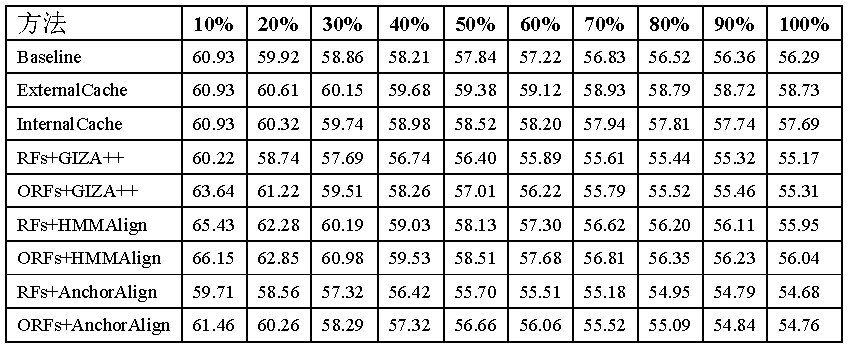
\includegraphics[width=\textwidth]{Figure/Table_5_1.pdf}
	\caption{译文质量随训练数据的增加的变化}
	\label{Table_quality_trainning_percent}
\end{table}

\begin{figure}[!bt]
	\centering
	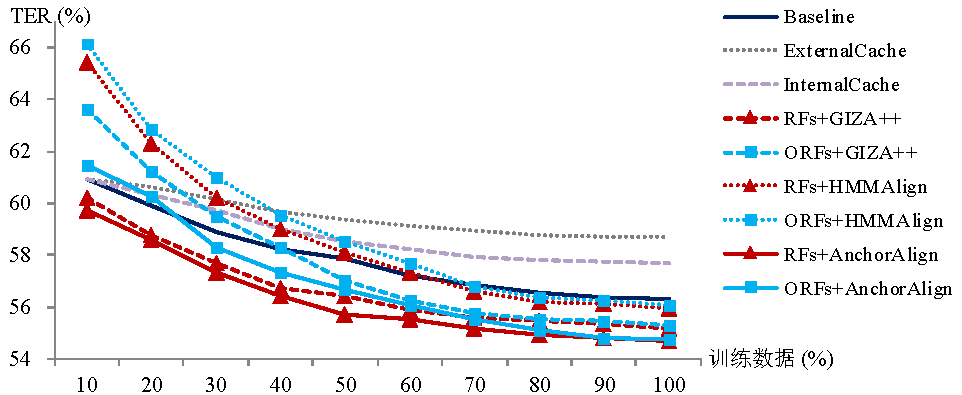
\includegraphics[width=0.98\textwidth]{Figure/Figure_5_6.pdf}
	\caption{译文质量随训练数据增加的变化的折线图}
	\label{Figure_quality_trainning_percent}
\end{figure}

\textbf{(1.2)词对齐方法对译文质量的影响}

词对齐方面,如果我们将短语翻译模型保持不变,如“ORFs”(█),就TER分值而言,带符号的实线代表的基于锚点的隐马尔可夫增量式词对齐方法(“Anchor-Align”)显著优于带符号的虚线代表的GIZA++,二者的TER分值相差约0.55个绝对百分点。我们也要看到,单独的基于隐马尔可夫模型的词对齐方法的翻译性能明显弱于GIZA++系统的。这意味着,通过将短语划分与词对齐任务进行联合以后,基于锚点的词对齐模型成功地提升了机器翻译译文质量。

如果我们仅关注基于锚点的增量式词对齐方法,相对于使用GIZA++的系统,使用基于在线随机森林的短语翻译模型的系统的TER值减少了0.49个绝对百分点。如果仅从TER值上讲,性能提升的效果是显著的。我们可以认为,基于锚点的隐马尔可夫增量式词对齐方法确实更适合基于在线随机森林的短语翻译模型进行在线学习。需要提及的是,GIZA++包括了基于隐马尔可夫模型在内的各种词对齐方法和优化方法的组合。因此,我们可以作如下结论:基于锚点的隐马尔可夫增量式词对齐方法显著提升了最终的机器翻译译文质量。

\textbf{(2)词对齐测试}

最后,我们单独测试不同方法对词对齐性能的影响。在词对齐实验中,训练数据为全部训练集,同时人工标注了测试集中的双语词对齐标准答案。表\ref{Table_word_alignment_compare}给出了完整的性能结果。“**”表示比基线系统在置信区间$p<0.01$显著提高。

\begin{table}[!htbp]
	\centering
	\begin{tabular}{|l|c|c|c|}
		\hline
		  & 准确率(\%) & 召回率(\%) & F值(\%) \\ 
		\hline
		GIZA++         & 71.42 & 75.73 & 73.51 \\ \hline
		HMMAlign       & 68.36 & 73.21 & 70.70 \\ \hline
		AnchorAlign    & \textbf{74.58**} & \textbf{80.92**} & \textbf{77.63**} \\ \hline
	\end{tabular}
	\caption{不同词对齐方法的性能结果}
	\label{Table_word_alignment_compare}
\end{table}

由表\ref{Table_word_alignment_compare}中的数据可知,相对于原始的隐马尔可夫词对齐模型和GIZA++而言,粗体数字表示我们提出的基于锚点的隐马尔可夫词对齐方法使双语词对齐的F值绝对值提高了超过4个绝对百分点,且统计显著。

综上所述,本文提出的基于随机森林的统计翻译在线学习方法能充分利用用户反馈的人工翻译句子,使机器翻译系统的译文质量得到稳步提升。

\section{本章小结}

机器翻译的在线自适应问题是人机交互式机器翻译不可忽视的重要问题。因为重复纠正相同错误的乏味感让使用机器翻译的专业译员感到沮丧。在本章中,我们提出了基于随机森林的统计翻译在线学习方法。该在线学习方法通过在人机交互过程中实时从输入源文和用户反馈构成的平行句对中抽取翻译知识,不断更新基于随机森林的统计翻译模型,从而改善译文的质量。由于低频词和未登录词直接影响词对齐和翻译知识抽取的性能,因此,我们还提出了一种基于锚点的隐马尔可夫增量式词对齐方法。该词对齐方法有效利用互信息和词典等先验知识生成对齐锚点,然后联合执行基于锚点的双语短语划分和隐马尔可夫词对齐算法。模拟实验结果表明,随着用户反馈的积累, 统计翻译在线学习方法显著提升了后续相关句子的自动译文质量,人机交互体验得到显著改善。该章介绍的工作是针对机器翻译在线自适应的一次成功尝试。